\chapter{Plotting with Scientific Python}

\section{Introduction}

This lab will highlight key Scientific Python features starting from
Python fundamentals.  It will introduce calculations and plotting
techniques using numpy arrays within Scientific Python.

\section{Starting a Jupyter notebook}

This course will make extensive use of the Jupyter Notebook interface
to Scientific Python, which is well suited to academic work (including
independent research) because it combines code with output in
digestable chunks.  Even when the end product is a polished peice of
software, much of the development occurs in the sort of interactive
sessions that Jupyter Notebooks provide.  

\begin{figure}[htbp]
\begin{center}
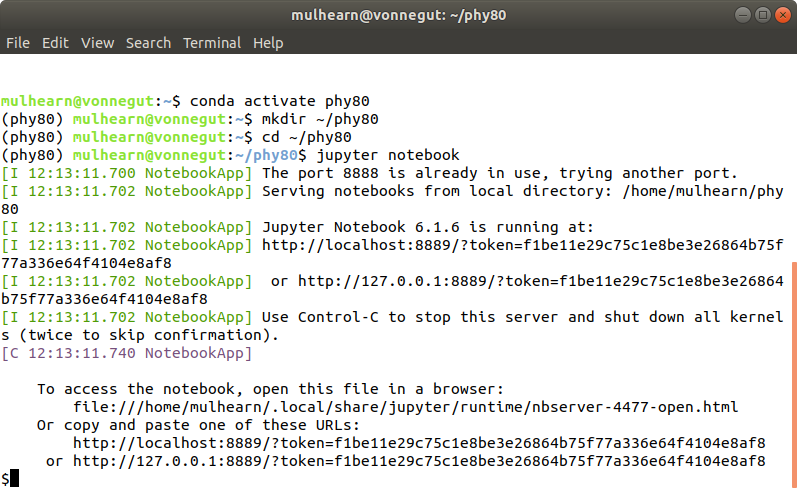
\includegraphics[width=0.65\textwidth]{figs/plotting/jupyter_startup.png} 
\caption{Example starting Jupyter Notebook from the Linux command line.  In Windows, you will need to open the Anaconda Prompt instead of a terminal.}
\label{fig:jupyterstartup}
\end{center}
\end{figure}

\begin{figure}[htbp]
\begin{center}
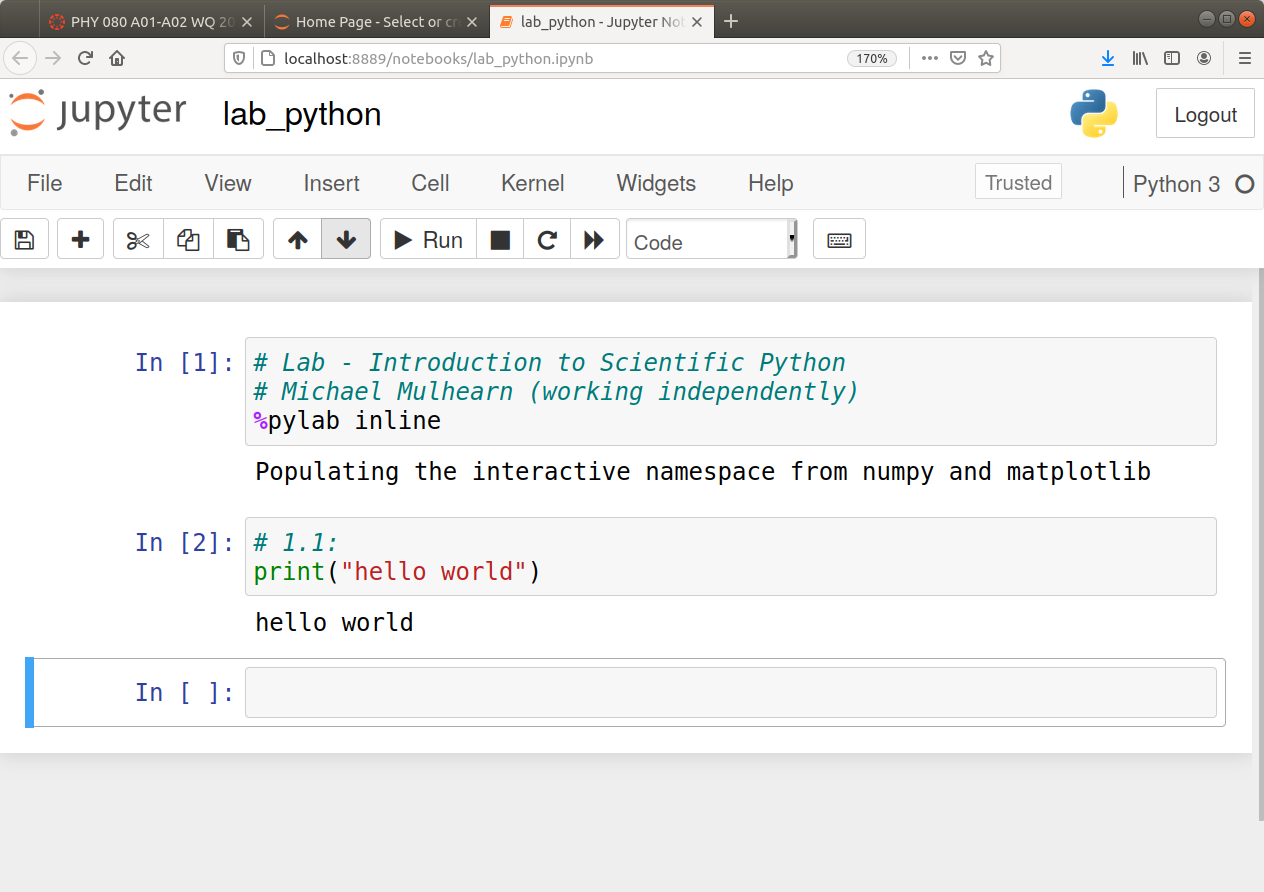
\includegraphics[width=0.65\textwidth]{figs/plotting/jupyter_window.png} 
\caption{The Hello World example Jupyter Notebook.}
\label{fig:jupyterwindow}
\end{center}
\end{figure}

\begin{figure}[htbp]
\begin{center}
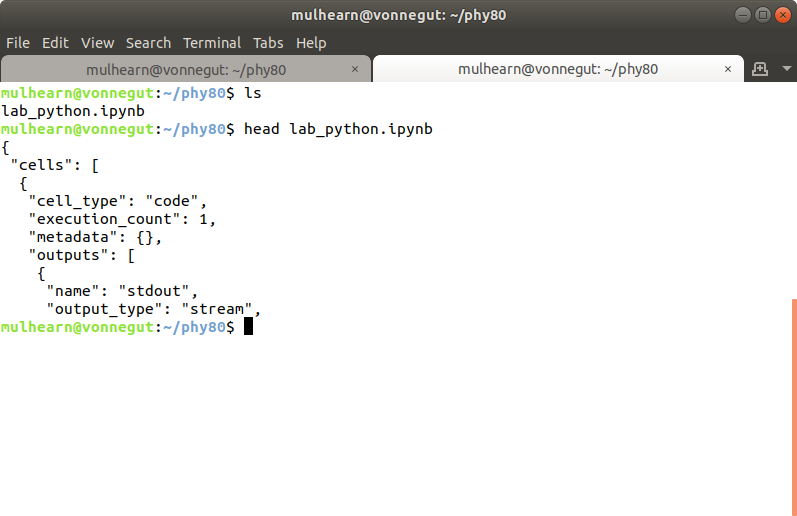
\includegraphics[width=0.65\textwidth]{figs/plotting/jupyter_saved.png} 
\caption{Example showing the saved Jupyter notebook.  Notice that notebook file (ipynb) is not human readable on its own: it requires the Jupyter software to render it in a human readable form.}
\label{fig:jupytersaved}
\end{center}
\end{figure}

After following the software installation instructions on the course
website, activate the Physics 80 environment with:
\begin{verbatim}
$ conda activate phy80
\end{verbatim}
Then, navigate to a working directory for this session, and start the notebook with:
\begin{verbatim}
$ jupyter notebook
\end{verbatim}
This should start the Jupyter Notebook server and open a client in your web browser.
An example starting a Jupyter Notebook from Linux is shown in Fig.~\ref{fig:jupyterstartup}.

You should create one Jupyter Notebook per lab assignment, by choosing
the New (Python 3) option in your client.  Change the name of your
notebook to something that clearly identifies the lab.  Start each lab
with comments (starting with ``\#'' symbol) indicating the title of
the lab, then your name followed by your lab partners.  See the first
cell of Fig.~\ref{fig:jupyterwindow} for an example.  This first cell
is also a good place to issue the ipython ``magic function'':
\begin{verbatim}
%pylab inline
\end{verbatim}
which will setup the notebook for inline plots and load the numpy and matplotlib libraries for you.

Each assignment will consist of a number of steps, clearly numbered like this one, you first step:

\begin{plot}
Print ``hello world'' using the python print command.
\end{plot}
\noindent
To keep your notebook clear, label cells (such as this one) with a
comment for the assignment step number, as in the second cell of
Fig.~\ref{fig:jupyterwindow}.  You only need to label one cell if
the assignment is fullfilled across several cells.

Jupyter Notebook checkpoints your work automatically.  You should be
able to see your notebook saved in the working directory where you
started, as in Fig.~\ref{fig:jupytersaved}.  Notice that while the
notebook file is ASCII text, it is not a human readable format.  The
Jupyter software is needed to render the notebook in a human readable
way.  To make your grader's life easier, you will be submitting PDF
versions of your notebook, once all of the tasks are completed and the
output is visible.  There are several ways to make a PDF file from
your notebook, but the most reliable is to use the ``Print Preview''
option to view the notebook as a PDF file within your browser, then
use the print feature of your browser to print the page as a PDF file.
Try this now, and make sure you can create a legible PDF file, but do
not submit it to the course site, as you still have more to do.
Always keep your python notebook file (ipynb) even after you submit
the assignment.  If you have problems, you can reproduce a PDF file
from the notebook file, but it is tedious to reproduce your notebook
from PDF.  If you have problems producing the PDF file, you can submit
the ``ipynb'' file as a temporary work-around, but work with your TA
to sort out the problem as quickly as possible.

\section{Scientific Python lecture notes}

A link to the Scientific Python lecture notes is available on the
course website.  These lecture notes are a community-based effort
which is well-maintained and constantly improving.  This section
contains example problems designed to reinforce the key concepts from
the first chapter of the Scientific Python Lecture Notes (SPLN).
Nearly all of Chapter 1 is useful, but these examples single out the
most essential sections for getting started with compuation in this
course.

Read through SPLN 1.2.2 and complete the following exercises in your notebook:

\begin{plot}
  Make some of your own simple calculations demonstrating the use of
  integers, floats, and Boolean variables.  Make your own list of
  strings, and demonstrate a few list operations.
\end{plot}

\begin{plot}
\begin{samepage}  
Try to predict the output of this code snippet:
\begin{verbatim}
a=3
b=a
a=2 #update
print(b)
\end{verbatim}
\end{samepage}
Run the code and check the output.  Are integers mutable or immutable?
At the line marked \#update, is a being changed by assignment or modification in place?
\end{plot}

\begin{plot}
Try to predict the output of this code snippet:
\begin{verbatim}
a=[3]
b=a
a[0]=2 #update
print(b[0])
\end{verbatim}
Run the code and check the output.  What type of data format is $a$?
Is that a mutable data type?  At the line marked \#update, is $a$
being changed by assignment or by modification in place?  Change that
line so as to do the opposite.  Does the program output change?
\end{plot}

Read through SPLN 1.2.3 and complete the following exercises in your notebook:

\begin{plot}
Use a for loop to print the first 10 powers of 3:  1,3,9,27,...
\end{plot}

\begin{plot}
Use a while loop to find the first number n for which the sum $1^2+2^2+3^2+...+n^2$ exceeds 1000.
\end{plot}

\begin{plot}
Use a for loop to calculate $n!$ by simply multiplying every value from $n$ to 1.
\end{plot}

\begin{plot}
Write a program to calculate and list the first 10 prime numbers after
100.  Use only basic python features such as while loops, for loops,
conditionals, assignment(=), equality (==), multiplication (*), and
the integer divide operation (//).  Do not use the mod operation (\%).
\end{plot}

Read through SPLN 1.4.1.1-3, 1.4.1.5 and complete the following problems:

\begin{plot}
Use the np.arange to define a 1-D numpy array of integers from 10 to
30 (inclusive).  Uses slices to print (a) every third element
(10,13,..), (b) the last five elements (26,27,...,30), and (c) every
other element in reverse order (30, 28, 26, ..., 10).
\end{plot}

\begin{plot}
Define variables $a$ and $b$ as numpy arrays of floats each of length
three.  Write a code snippet to calculate and print the vector dot
product of $a \cdot b$ using an explicit for loop, i.e. loop over
indexes 0,1,2 and increment a sum by the product.  This is how you
write this program in a language such a C.  Now use the python * and
np.sum operation to compute the dot product in a single line, with no
explicit for loop.  The elimination of tedious explicit for loops is
why programming in Scientific Python is much more fun than any other
common language, once you get used to the idea.
\end{plot}

The Scientific Python Lecture Notes are an excellent resource.  These
examples and sections are a good starting point for the work we will
be doing in this course, but remember that there is much more
available for you to refer to in the future!

\section{Plotting discrete data and continuous functions}

\begin{figure}[htbp]
\begin{center}
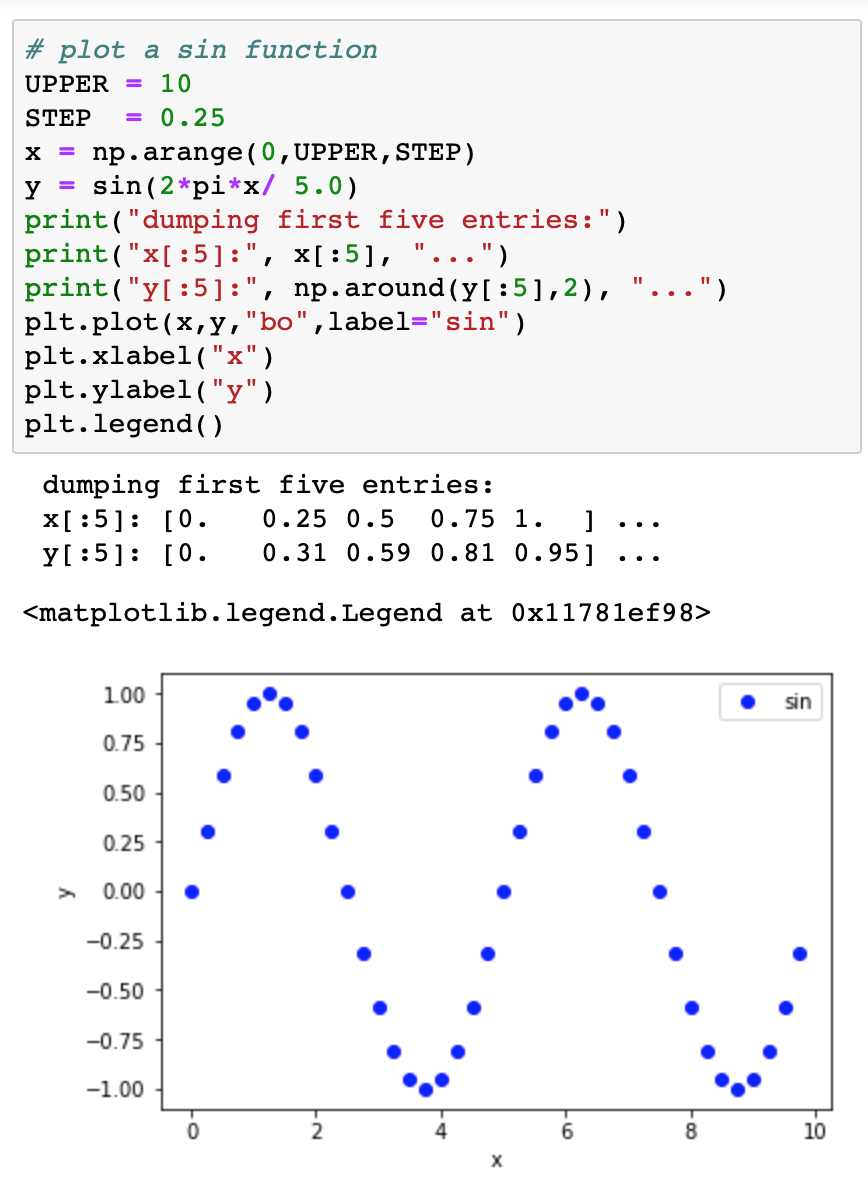
\includegraphics[width=0.65\textwidth]{figs/plotting/plotting.png} 
\caption{Sine function sampled at discrete values.}
\label{fig:plotsin}
\end{center}
\end{figure}

Consider the Jupyter Notebook example in Fig.~\ref{fig:plotsin} which
plots a sine function sampled at discrete values.  Note the following
key features, which you will use repeatedly today and in future labs:
\begin{itemize}
\item Use of global variables {\tt UPPER} and {\tt STEP} at the top of the snippet, allowing for easy adjustment of parameters that affect the plot.
\item Use of {\tt np.arange} to define an array of x values.
\item Creation of the array y, defined by $y = \sin(2\pi x / 5)$ for each value of x.  One of the great joys of using numpy is the ability to avoid getting bogged down with explicit for loops.
\item Use of slicing techniques {\tt x[:5]} to show only the first five entries for debugging.  
\item Plotting the arrays of $x$ and $y$ values with {\tt plt.plot}  using the {\tt "bo"} option for blue circles.
\item Defining appropriate axis labels with {\tt plt.xlabel} and {\tt plt.ylabel}. 
\item Creation of a legend using the {\tt label} option to {\tt plt.plot} and the {plot.legend()} command.
\end{itemize}
Notice that even in this simple example, I've added some intermediate
feedback from my code in the form of the screen dumps of the first few
values of $x$ and $y$.  It's a common pitfall to try and rush ahead to
the final product when programming.  But it is much faster and
reliable to break your task into small steps, and establish feedback
at each small step.

To plot a continuous function with Scientific Python, you will still
use discrete data but:
\begin{itemize}
 \item Use much finer binning of the $x$-axis variable to draw a smooth curve. 
 \item Use the line option {\tt "-"} or dashed line {\tt "--"} instead of points with {\tt "o"}. 
\end{itemize} 

\noindent
%{\bf Plot 1:}  
\begin{plot} \end{plot}
Plot the sinc function with the following requirements:
\begin{itemize}
 \item Plot in the range $x = (-5,5)$.
 \item Plot discrete samples with a step size of $0.5$ using blue circles.
 \item On the same axis, plot the corresponding smooth function using
   a red solid line.  The smooth function should use much finer
   binning to approximate a continuous curve.
 \item Add appropriate axis labels. 
 \item Add a legend for the ``discrete'' and the ``smooth''  function.
\end{itemize}
Use the numpy sinc function, e.g. {\tt y = np.sinc(x)}.


\section{Multivariate analysis using boolean masks}
\begin{figure}[htbp]
\begin{center}
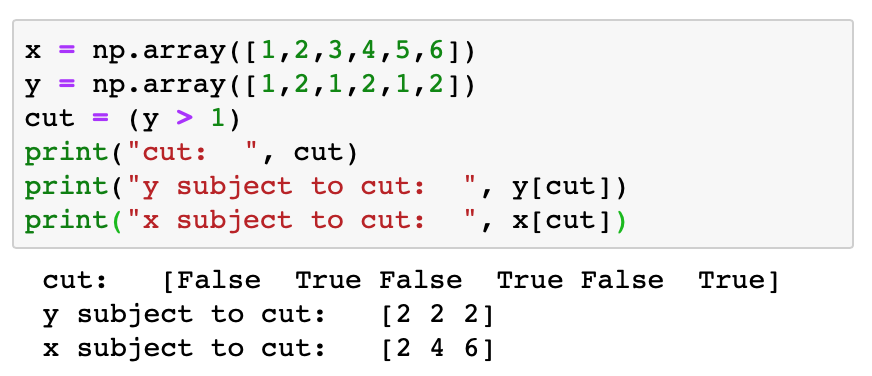
\includegraphics[width=0.65\textwidth]{figs/plotting/booleanmasks.png} 
\caption{Using boolean masks to cut on variable $y$.}
\label{fig:booleanmasks}
\end{center}
\end{figure}

A powerful technique in Scientific Python for performing analysis
involving multiple variables uses boolean masks as shown in
Fig.~\ref{fig:booleanmasks}.  In the example:
\begin{itemize}
\item Two numpy arrays $x$ and $y$ {\tt of the same length} are defined to contain the collected data.
\item The cut defined by $y > 1$ is a boolean array of the same length as $x$ and $y$ which is true at indices where the condition is met and false where it is not.
\item The subset of the entire $y$ array defined by {\tt y[cut]} consists only of those entries of $y$ for which the condition $y>1$ is met.
\item The subset of the entire $x$ array defined by {\tt x[cut]} consists only of those entries of $x$ for which the condition $y>1$ is met for the corresponding y value.
\end{itemize}
The last item shows the real power of this technique, one can look at one variable subject to constraints on another variable.

\begin{table}
\caption{Sample data for a voltage measurement subject to high frequency noise.}
\label{tbl:hfnoiseeg}
\begin{center}
\begin{tabular}{lll}
$t~(\rm s)$ & $v~(\rm V)$ & $n$ \\
0.4  & 0.25  &  2.8 \\
1.1  & 2.37  &  7.3 \\
1.4  & 1.69  &  9.7 \\
1.9  & 0.93  &  1.3 \\
2.5  & -1.0  &  6.2 \\
3.0  & 0.95  &  4.8 \\
3.4  & 1.22  &  6.9 \\
4.1  & 0.54  &  4.0 \\
4.4  & 0.37  &  1.9 \\
4.8  & 0.13  &  4.0 \\
5.5  & -2.04  &  9.5 \\
6.2  & -2.06  &  8.7 \\
6.5  & -0.81  &  2.3 \\
7.0  & -0.95  &  5.3 \\
7.5  & 0.98  &  9.7 \\
7.9  & 0.27  &  8.3 \\
8.5  & -0.81  &  0.1 \\
9.0  & -0.59  &  5.1 \\
9.4  & -0.37  &  4.4 \\
9.9  & 0.56  &  9.9 \\
\end{tabular}
\end{center}
\end{table}

Next consider the sample data in Table~\ref{tbl:hfnoiseeg} which comes
from experimental measurements of a voltage level $v$ at discrete
times $t$.  The measurement is subject to a high-frequency noise
monitoring by the variable $n$.  The noise is only present for $n >
6.0$.  A straightforward way to load this data into scientific python
is by defining numpy arrays for each variable as follows:
\begin{verbatim}
t = np.array([0.4, 1.1, 1.4, 1.9, 2.5, 3.0, 3.4, 4.1, 4.4, 4.8, 
                     5.5, 6.2, 6.5, 7.0, 7.5, 7.9, 8.5, 9.0, 9.4, 9.9])
v = np.array([ 0.25, 2.37, 1.69, 0.93, -1.0, 0.95, 1.22,   
                      0.54, 0.37, 0.13, -2.04, -2.06, -0.81, -0.95,  
                      0.98, 0.27, -0.81, -0.59, -0.37, 0.56])
n = np.array([2.8, 7.3, 9.7, 1.3, 6.2, 4.8, 6.9, 4.0, 1.9, 4.0,  
                      9.5, 8.7, 2.3, 5.3, 9.7, 8.3, 0.1, 5.1, 4.4, 9.9])
\end{verbatim}

\noindent
%{\bf Plot 2} 
\begin{plot} \end{plot}
Prepare a plot of the sample data subject to the following:
\begin{itemize}
 \item Plot the voltage as a function of time as discrete data using red points.
 \item Define the boolean array {\tt keep} based on the noise reducing condition $n<=6.0$.
 \item Plot the voltage as a function of time, subject to the noise reducing condition using blue points.
 \item Plot the function $\sin(2 \pi x / 10)$ as a smooth function.
 \item Add appropriate axis labels.
 \item Add a legend for ``raw'' data with no cut, ``clean'' data with noise removed, and your continuous ``sin'' function.   
\end{itemize}
Your plot will reveal a clear sine function in the discrete data
(after noise removal) consistent with the continuous function.  {\bf
  This is a sign-off point for the lab.}

\section{The Logistics Map}
The logistics map is the recurrence relation
\begin{displaymath}
x_{n+1} = r \, x_n \, (1 - x_n)
\end{displaymath}
with the variable $x$ between $0$ and $1$.  The variable $x$ can be
thought to represent the ratio of a population to its maximum possible
value.  The population increases due to birth and decreases due to
starvation as the population approaches it's maximum value ($x$ near
1).  This leads to the non-linear relationship that defines the
logistic map.  The mapping keeps the variable x between $0$ and $1$ as
long as the parameter r is in the range $[0,4]$.

The logistics map is frequently encountered as a simple example of a
chaotic system emerging from a simple non-linear system.  If we
consider the long term behavior of the population $x$ as a function of
the parameter $r$, as shown in Fig.~\ref{fig:logmap}, we see that for
values of $r$ less than $3$ the population approaches a single fixed
value.  At the value $r=3$ the non-linear system exhibits bifurcation
with the population oscillating between two values.  As $r$ increase,
further bifurcations occur at an ever increasing rate until the
systems exhibits chaotic behavior alternating with occasional returns
to stable oscillations.

\begin{figure}[htbp]
\begin{center}
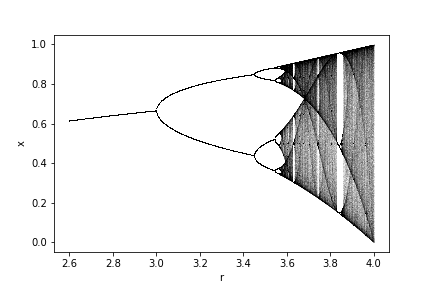
\includegraphics[width=0.65\textwidth]{figs/plotting/bifurcation.png} 
\caption{Long term behavior of the logistics map.}
\label{fig:logmap}
\end{center}
\end{figure}

\begin{figure}[htbp]
\begin{center}
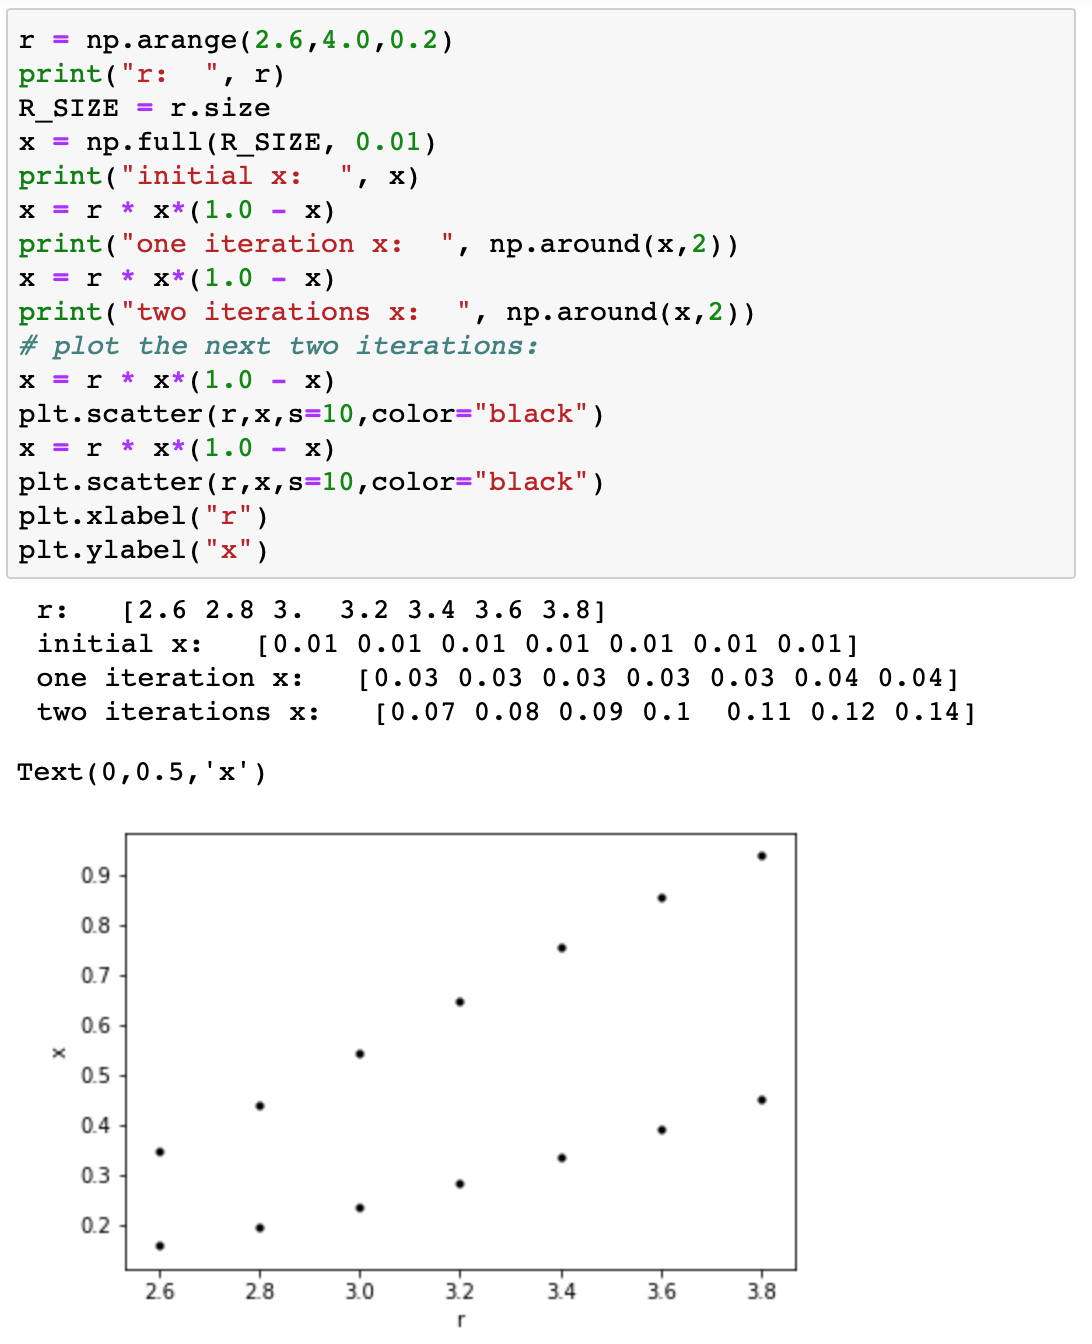
\includegraphics[width=0.85\textwidth]{figs/plotting/logmapstart.png} 
\caption{Modeling the logistics map.}
\label{fig:logmapstart}
\end{center}
\end{figure}

The long term behavior of the logistics map can be easily modeled in
Scientific Python.  A start is shown in Fig.~\ref{fig:logmapstart}
where you should understand:
\begin{itemize}
\item An array of $r$ values is defined.
\item An array of $x$ values of the same size as $r$ is defined and initialized to an arbitrary non-zero value (0.01).
\item Two example iterations of the logistic map are applied.
\item The next two iterations of the values of $x$ are plotted as function of $r$ on the same plot.
\end{itemize}

\noindent
%{\bf Plot 3:} 
\begin{plot} \end{plot} Reproduce the figure in Fig.~\ref{fig:logmap} by doing the following:
\begin{itemize}
\item Define two global variables {\tt ITER = 10} and {\tt PLOT = 5}.
\item Apply the logistics map {\tt ITER} times by using a for loop.
\item Apply the logistics map an additional {\tt PLOT} times, plotting the values of $x$ as a function of $r$, as in the example, each time.
\end{itemize}
You'll observe the long term behavior by increasing the value of {\tt
  ITER} to a large value, such as 10,000.  You'll see the full
dependence on $r$ by decreasing the step size in the initialization of
the numpy array $r$ to something like $0.001$.  You'll observe the
chaotic behavior by increasing the value of {\tt PLOT} to 100 or even
1000 iterations.  To make a prettier plot using finer points (once you
have a large number of points) you can reduce the size by adjusting
the {\tt s=10} parameter in the call to {\tt plt.scatter} to something
like {\tt s=0.0001}.

\section{Submitting your assignment}

Before submitting, take some time to clean up your assignments to
remove anything superfluous and place the exercises in the correct
order.  You can also add comments as needed to make your work clear.
You can use the Cell $\to$ All Output $\to$ Clear and Cell $\to$ Run
All commands to make sure that all your output is up to date with the
cell source.

When you are satisfied with your work, print the PDF file as described
earlier and submit it to the course website.

